\documentclass[12pt]{article}
\usepackage[T1]{fontenc}
\usepackage[utf8]{inputenc}
\usepackage[francais]{babel}
\usepackage{graphicx,float}
\usepackage{algorithm, algorithmic}
\usepackage{verbatim}
\usepackage{listings}

\floatname{algorithm}{Algorithme}
\renewcommand{\algorithmicrequire}{\textbf{Entrée :}}
\renewcommand{\algorithmicensure}{\textbf{Sortie :}}
\renewcommand{\algorithmicend}{\textbf{fin}}
\renewcommand{\algorithmicif}{\textbf{si}}
\renewcommand{\algorithmicthen}{\textbf{alors}}
\renewcommand{\algorithmicelse}{\textbf{sinon}}
\renewcommand{\algorithmicfor}{\textbf{pour}}
\renewcommand{\algorithmicforall}{\textbf{pour tout}}
\renewcommand{\algorithmicdo}{\textbf{faire}}
\renewcommand{\algorithmicwhile}{\textbf{tant que}}
\renewcommand{\algorithmicloop}{\textbf{boucle}}
\renewcommand{\algorithmicrepeat}{\textbf{repéter}}
\renewcommand{\algorithmicuntil}{\textbf{jusqu'à}}
\renewcommand{\algorithmicprint}{\textbf{afficher}}
\renewcommand{\algorithmicreturn}{\textbf{retourner}}
\renewcommand{\algorithmictrue}{\textbf{vrai}}
\renewcommand{\algorithmicfalse}{\textbf{faux}}

\begin{document}
\title{Tracage UltraSonic : Reverse Engineering d'une application Android}
\author{Benoit BILLAUDEL}

\maketitle

\section*{Introduction}
Lorem ipsum dolor sit amet, consectetur adipiscing elit, sed do eiusmod tempor incididunt ut labore et dolore magna aliqua. Ut enim ad minim veniam, quis nostrud exercitation ullamco laboris nisi ut aliquip ex ea commodo consequat. Duis aute irure dolor in reprehenderit in voluptate velit esse cillum dolore eu fugiat nulla pariatur. Excepteur sint occaecat cupidatat non proident, sunt in culpa qui officia deserunt mollit anim id est laborum.

\section{Traitement du Signal}
Le son est une onde mécanique. Une onde se présente comme vibration du millieu dans lequel elle se propage, en l'occurence l'air.
Une onde se propage de manière continue dans la nature, elle est dite analogique. Une onde sonore simple peut être modélisée par une sinusoïde, on parlera ainsi de l'amplitude et de la fréquence de l'onde comme l'amplitude et la fréquence de la sinusoïde. L'amplitude se mesure en Pascal (Pa) et la fréquence en Hertz (Hz).

On parlera de sons pure (ou sons simple) quand le son n'est composé que d'une seul fréquence avec un amplitude constante au cours du temps, un exemple est le diapason qui produit un "la" pure à 440Hz.
Dans la nature il est très rare de rencontrer des sons pure, on fréquente plutôt des sons complexes qui sont composés de plusieurs sons pure de fréquences et d'amplitudes différents

Un émetteur tout comme un capteur de sons sont donc des corps vibrant à un certaine fréquence. Dans le cas de l'Homme les corde vocales vibrent pour produire des sons et les tympants vibrent pour les transcrire en information que le cerveau pourra interpréter. Dans le monde numérique, une enceinte fonctionne de la même manière, elle est munie d'une membrane qui vibrera à la manière des cordes vocales, de même pour un micro ou l'air fera vibrer une membrane et un capteur traduira la vibration de la membrane pour le cerveau. La Fréquence est donc la vitesse à laquelle la membrane change d'état. l'amplitude est la différence de position de la membrane au repos et de sa position quand elle est soumit a un son.

Un ordinateur n'est pas capable de traiter des signaux analogiques, il faut donc discretiser ce signal. On parlera d'échantillonage. c'est à dire qu'on ne prendra que des valeurs instantané de la sinusoïde, des échantillons, pour en obtenir une approximation. La fréquence a laquelle ces échantillons sont pris se nomme la fréquence d'échantillonage, et par extension plus elle est élevée plus le sons digital sera de bonne qualité. 
\begin{figure}[H]
\begin{center}
\caption{différence entre un signal Analogique et Digital}
\label{fig:analogDigit}
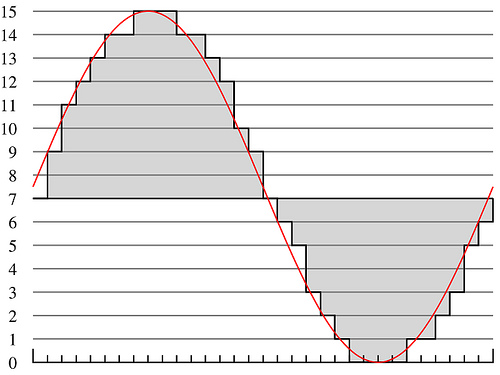
\includegraphics[scale=0.5]{analogique-digital.jpg}
\end{center}
\end{figure}
La loi de Shannon nous dit : \emph{\og La représentation discrète d'un signal exige des échantillons régulièrement espacés à une fréquence d'échantillonnage supérieure au double de la fréquence maximale présente dans ce signal. \fg{} }
L'oreille humaine est en théorie capable d'entendre les fréquences de 20Hz à 20kHz, en pratique il est très rare d'être capable d'entendre clairement au delà 17-18kHz.
Dans le commerce la fréquence d'échantillonge la plus commune, celle des CD est de 44100Hz, avec un spectre allant de 0Hz a 22050Hz, largement suffisant donc pour l'oreille humaine.

Le traitement du signal regroupe toutes les methodes et outils utilisés pour traiter un signal. Le but étant de se servir d'un onde comme support au transport d'information. 

\subsection{Modulation d'amplitude et Modulation de frequence}
La modulation et la démodulation d'un signal sont deux étapes pour la transmission d'une information, le signal étant rarement adpaté a la transmission direct par le canal de communnication choisi.
La modulation permet donc de translater le spectre du message dans un domaine de fréquences qui est plus adapté au moyen de propagation et d'assurer après démodulation la qualité requise par les autres couches du système. Il existe deux pricipales methodes de modulation, la modulation d'amplitude et de fréquence.

La modulation d'amplitude (AM, cf Figure~\ref{fig:modAmp}) consiste à faire varier l'amplitude d'un signal de fréquence élevée, le signal porteur, en fonction d'un signal de plus basse fréquence, le signal modulant. Ce dernier est celui qui contient l'information à transmettre. c'est la methode de modulation la plus simple a mettre en place. Elle a été historiquement utilisée pour la radiodiffusion.
\begin{figure}[H]
\begin{center}
\caption{Exemple de modulation d'amplitude}
\label{fig:modAmp}
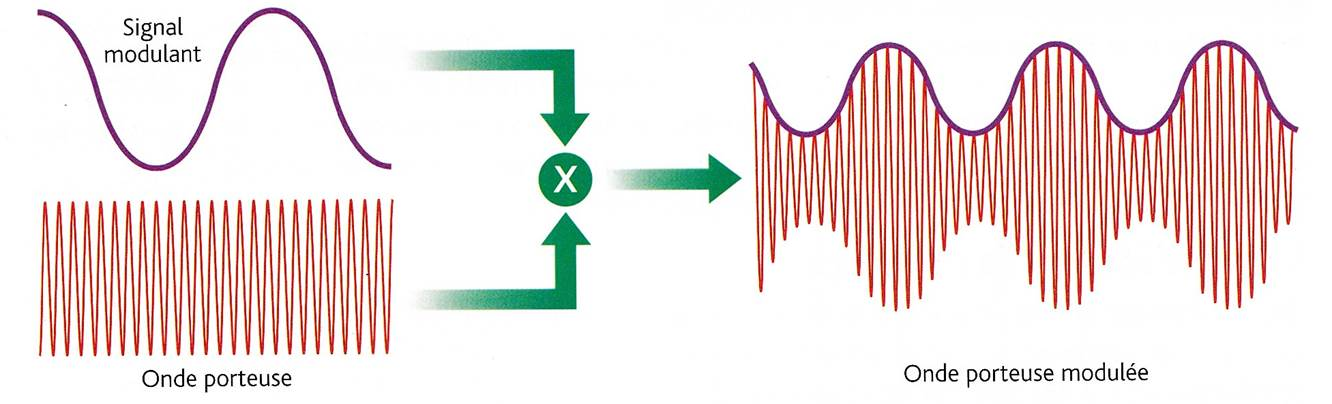
\includegraphics[scale=0.30]{modAmp.jpg}
\end{center}
\end{figure}

La modulation de fréquence (FM, cf Figure~\ref{fig:modFreq}) est un mode de modulation consistant à transmettre un signal par la modulation de la fréquence d'un signal porteur (porteuse).
En modulation de fréquence, l'information est portée par une modification de la fréquence de la porteuse, et non par une variation d'amplitude. La modulation de fréquence est plus robuste que la modulation d'amplitude pour transmettre un message dans des conditions difficiles (atténuation et bruit importants).
\begin{figure}[H]
\begin{center}
\caption{Exemple de modulation de fréquence}
\label{fig:modFreq}
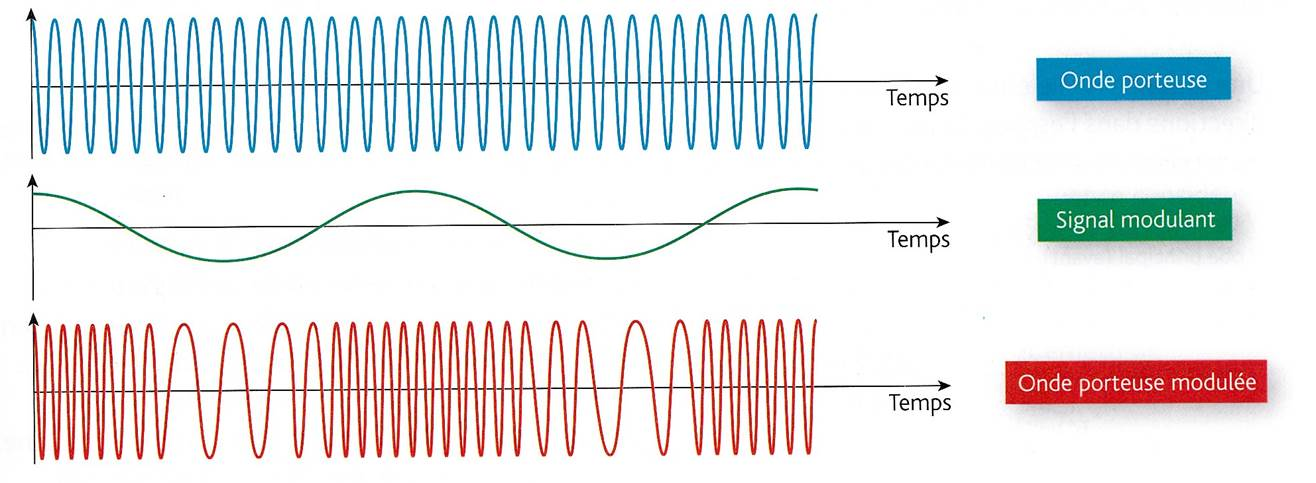
\includegraphics[scale=0.30]{Mod_Freq.jpg}
\end{center}
\end{figure}

Il est donc possible de coder de l'information dans une onde, en l'occurence sonore.
La modulation de fréquence étant plus robuste, on préfèrera utiliser cette methode.

\subsection{Transformé de Fourier Discrète}
La transformé de Fourier discrete est un outil mathématique en traitement du signal. À partir d'un ensemble d'échantillons du signal, il permettra de calculer un nombre proportionnel à l'amplitude d'une bande de fréquences spécifique. on pourra ainsi établir si cette bande de fréquences est présente majoritairement ou non dans le signal.\\

un implémenttation de la transformé de fourrier naïve sera :
\begin{verbatim}
def fourierNaif(data):
	omega = 2*np.pi*FreqCherche/SampleRate
    eiw = complex(numpy.cos(omega), numpy.sin(omega))
    f = 0
    for s in data:
        f = eiw*f + s
    return f
\end{verbatim}

Le signal entrant est automatiquement converti en échantillons par le micro. On utilisera un algorithme Pour calculer la transformé de Fourier pour traiter ce signal. Il en existe plusieurs, les plus connus étant l'algorithme de Goertzel et la transformé de Fourier Rapide (FFT).

On traite les échantillons par bloc, chaque bloc étant un ensemble d'échantillon, plus il est grand plus le résultat sera précis, mais plus le calcul sera plus lourd.
\begin{algorithm}[H]
\caption{Goertzel}
\begin{algorithmic}
\REQUIRE{$X$ le tableau d'echantillons de longueur $N$, $F$ la fréquence à detecter et $S$ la fréquence d'échantillonage}
\ENSURE{$A$ la valeur associé à l'amplitude de $F$}
\STATE{$k = ($int$)(0.5+N*F/S)$}
\STATE{$\omega = k * (2*\pi/N)$}
\STATE{$c = 2* \cos(\omega)$}
\STATE{$q_1 = q_0 = 0$}
\FOR{$i$ de 0 à $N-1$}
\STATE{$q_0 = c* q_1 - q_2 + X[i]$}
\STATE{$q_2$ = $q_1$}
\STATE{$q_1$ = $q_0$}
\ENDFOR
\STATE{$A = q_1^2 + q_2^2 - q_1*q_2*c$}
\RETURN{$\sqrt{A}$}
\end{algorithmic}
\end{algorithm}

En sortie on récupèrera la valeur associée à l'amplitude de la fréquence recherché qui, si elle est au dessus d'un certain seuil, peut être considéré comme présente dans le signal initial. Ce seuil dépendra de la qualité de l'émeteur, de celle du capteur ainsi que de l'environement.
En pratique pour traiter avec seulement certaines fréquences spécifiques, la methode naïve est suffisante.

\subsection{Balise ultrasonique (uBeacon)}
L'oreille humaine est supposé être capable d'entendre les frequences entre 20Hz et 20 kHz. En réalité l'oreille n'est que rarement capable d'aller au delà des 18kHz.\\
Pour cela le terme "ultrasonique" désigant les fréquences supérieur à 20kHz, est ici un abus de langage. en Réalité une uBeacon est un message encodé dans des fréquences comprises entre 18kHz et 20kHz et donc quasi-inaudible. Comme on l'a vu précedement on sera capable de récupérer cette balise à l'aide de la transformé de fourier.

Ainsi une methode simple sera la modulation par déplacement de frequences (ou Frequency Shift Keying FSK, cf Figure~\ref{fig:fskExemple}) c'est à dire de définir deux fréquences (0 et 1), de definir un nombre d'échantillons comme la longueur d'un bit. On peut ainsi encoder un message binaire caché dans un signal sonore en faisant alterner les deux fréquences.

\begin{figure}[H]
\begin{center}
\caption{Exemple de FSK}
\label{fig:fskExemple}
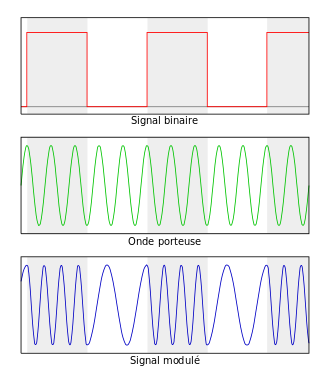
\includegraphics[scale=0.75]{FSK.png}

\tiny{source : wikipedia}
\end{center}
\end{figure}
 
L'inconvénient majeur de cette methode pour transmettre un message, est qu'avant de pouvoir traiter le signal, se synchroniser avec lui.

Il existe plusieurs méthodes de synchronisation, celle présenté suis l'intuition la plus simple. on admet que le premier bit à recevoir est un 1 et la longueur d'un bit est de $L$ échantillons, on cherche donc à se synchroniser avec la $F_1$ la fréquence associé à un 1 logique (en vert, cf : Figure~\ref{fig:syncro}).
On considèrera que les échantillons arrivent les un après les autres dans la mémoire. On prendra un buffer de $3*L$. On appliquera Goertzel sur les échantillons $L$ à $2*L$. Après avoir identifié la présence de $F_1$, il faut s'aligner avec. Pour ce faire, il suffira d'appliquer Goertzel de l'échantillon $i$ à $L+i$ pour $i \in [0,2*L]$ et de chercher dans lequel de ces blocs d'échantillons $F_1$ est la plus forte .

\begin{figure}[H]
\begin{center}
\caption{Synchronisation}
\label{fig:syncro}
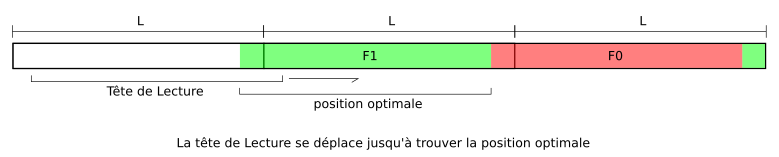
\includegraphics[scale=0.8]{syncro.png}
\end{center}
\end{figure}

En générale le message sera précédé d'un séquence de bit standardisé permettant la syncronisation, puis un séquence pour vérifier que la synchronisation est correcte.

Dans la pratique la portion du spectre sonore 18-20kHz sera découpé en +/- 26 fréquences auxquels seront attribuées une lettre.

Une balise sera une combinaison des ces lettres, sans soucis d'ordre et sans répétition de lettres. on construira la balise avec les fréquences correspondantes à chaque lettre, qui seront mixés ensemble, et cachés dans un fichier audio par exemple.

L'interêt de cette methode est que, contrairement à la première, il n'y a pas à se soucier de la synchronisation entre l'émeteur et le capteur. Il suffiera d'envoyer en continu pendant un temps suffisemant long la balise et de la traduire. En revanche l'ensemble des messages possibles est bien plus limité.

\section{Écosystème Android et Reverse Engineering}

\subsection{Écosystème Android}
Dans cette partie nous allons nous interresser à certains outils que nous fournis Android.

Android étant développé en Java, et selon la devise de java \textit{\og write once, run anywhere\fg{}} il a besoin d'un machine virtuelle java pour fonctionner, en l'occurence celle d'Android se  nommait \og Dalvik \fg{}. Elle est en mesure de traiter des fichier .dex et .odex (Dalvik EXecutable et Optimized DEX) qui sont une sorte de .jar consolidé et optimisés pour Android.

depuis la version 5.0 "Lollipop" d'Android, Dalvik est entièrement remplacé par ART (Android Runtime)~\cite{ART}. ART utilise la compilation anticipée, en compilant l'application à son installation, sans besoin ultérieur d'interprétation. ART permet ainsi d'augmenter les performances, donc d'augmenter la durée de vie de la batterie. De plus les allocations mémoires sont plus efficace. Dans un soucis de rétro-compatibilité, ART utilise toujours des fichiers .dex, mais pas de .odex, qu'il remplace par des fichier ELF (Executable and Linkable Format)

Il est important de noter qu'une application Android se présentera toujours sous forme d'une archive .apk. Cette archive contiendra entre autres le fichier AndroidManifest.xml sur lequel nous nous attarderons par la suite, un fichier classes.dex et enfin les ressources de l'application c'est à dire les images, musiques et autres éléments nécessaire à l'application.

\subsubsection{Intents}
Les intents sont un format de message d'action spécifique à Android. Un intent est composé de plusieurs champs : 
\begin{itemize}
\item un champ \textit{action} qui défini quel type d'action sera à executer
\item un champ \textit{data} qui contiens les éventuelles données nécessaire à l'action
\item un champ \textit{category} qui donne plus d'information sur l'action
\item un champ \textit{type} qui spécifie le type de donnés du champs \textit{data}
\item un champ \textit{component} qui spécifie la class qui résulura l'intent
\item un champ \textit{extras} qui contiendra des éventuelles information ou données complémentaire
\end{itemize}

Il existe deux type d'intents, les intents explicites et implicites.

Les intents explicites sont destinés a un composant spécifique de l'application, et donc à une classe précise qui sera en charge de le résoudre. C'est en général de cette manière qu'une application lancera des activitées après une interaction avec l'utilisateur.

Les intents implicites en revanche ne sont pas destinés à un composant spécifique, mais ils doivent contenir suffisement d'information pour que le système puisse déterminer quel composant sera le plus en mesure de le résoudre.

Le système Android envoie frequement des intents implicites, des <<Broadcast>>, qui seront entre autre gérés par des classes \textit{BroadcastReceiver}. Ces intents servent en générale a communiquer aux application l'état de l'appareil, par exemple si la connexion réseau est active, ou si la batterie est presque vide.

\subsubsection{Manifeste Android}
Une application contient obligatoirement un fichier AndroidManifest.xml. Ce fichier fourni des informations au système Android, information nécessaire avant de pouvoir executer le code.

Entre autre, il sert à :
\begin{itemize}
\item nommer le package Java. ce nom servira d'identifiant unique a l'application.
\item décrire les composants de l'application, c'est à dire les activitées, les services les broadcast receivers, ainsi que les nom des classes qui implémentent chacun de ces composants.
\item établie les liens entres les Broadcast système et les Broadcast receiver.
\item déclare les permission requises pour l'application.
\item déclare la version minimum de l'API Android nécessaire pour faire marcher l'application
\item liste les bibliothèques auxquels ai liée l'application
\end{itemize}

Comme vu précédement, la plupars des composants d'une application Android sont activés par des intent. La section <intent-filter> du manifeste servira donc à signaler au système quel composant est capable de gérer quel intent, en sachant que chaque composant peux gérer plusieurs intent.

De même les permission sur les sytème Android, servant a protéger les données ou éléments dits critiques, sont à définir dans le manifeste. Ainsi a l'installation, si nécéssaire le système demandera à l'utilisateur si il accepte que l'application accède a tel ou tel focntionalité de l'appareil. À noter que dans les dernières version d'Android, un application pourra fonctionner, dans la mesure du possible, si certaines des permissions qu'elle demande lui sont refusées.

\subsection{Écosystème de Reverse Engineering}
Il existe plusieurs outils de rétro-ingénierie pour les systèmes Android notamment Androguard, Apktool, Radare2...

En raison des contraintes imposées par le hardware ou par la volonté de portabilité d'une application, une methode commune, pour developper une application lourd en puissance de calcul ou en espace mémoire, sera d'ulitilser un langage natif comme le C/C++. En effet C/C++ est bien plus souple que Java en terme d'optimisation mémoire.

En revanche beaucoup de décompilateurs Java ne sont pas capable de comprendre le C/C++ et donc d'autres methodes seront nécessaire pour récuperer le code source de ces applications.

Androgurad est un outil en Python capable de traiter des archives DEX, ODEX, APK, les fichiers XML, les ressources android. Il est aussi capable de dessassembler ou décompiler des fichier DEX/ODEX.

Apktool propose plus ou moins les mêmes fonctionalitées, il permet en plus de reconstruire des ressources en APK/JAR. Il permet aussi l'utilisation de smalidea, un langage plugin d'Itellij IDEA et de Android Studio, premettant ainsi d'accéder à un debbugeur.


\subsection{Application}

A REFAIRE/COMPLETER\\

\og Bird Up Up \fg{} était un jeu assez simpliste. le but est de farie sauter un oiseau le plus haut possible en tapant sur l'écran au bon moment, le tout en évitant des obstacles. Ce jeu n'est plus disponible sur le Google play store.
Cette application a été identifié~\cite{silverpushunmasked} comme utilisant le SDK de Silverpush, connu pour implmenter des methodes de tracage ultrasonique des utilisateurs et des appareils.

Pour la retro-ingenerie de l'application, après avoir récupéré le code source sorti du décompilateur, on peut commencer par observer le manifeste android de l'application. Dans le cas de Bird Up Up, on voit que les intents ACTION\_BATTERY\_OKAY et ACTION\_BATTERY\_LOW sont liées a un Broadcast receiver. L'intent Battery\_LOW est émit quand le niveau de la batterie descend en dessous de 10\%. Or on sait que le traitement d'une uBeacon peut être lourd et donc le lier à l'état de la batterie peut s'avérer judicieux.

En allant observer le code source du broadcast receiver lié aux intents on observe qu'il lance ou tue le service d'écoute via la classe Silverpush.class.
Pour ce faire il fait appel à la methode methode getInstance(). En cherchant simplement cet appel dans l'intégralité du code source, en utilisant grep par exemple, on observe que cet appel est aussi fait dans une autre classe, qui par la suite initialisera et lancera le service d'écoute.

On est maintenant capable d'établir un schema de fonctionnement grossier

\newpage
\bibliography{bibli}
\bibliographystyle{abbrv}
\end{document}